% Presetting

    \documentclass[11pt]{book}

    \RequirePackage{silence}
    \WarningFilter{remreset}{The remreset package}

    % Chapter Style

            % Headings  
            \usepackage[Glenn]{fncychap}
            \ChNumVar{\fontsize{40}{42}}
            \ChTitleVar{\Large\sc}
            \ChNameVar{\empty}
            \setlength\headheight{14.5pt}
            
            % Roman Numerals
            \usepackage{remreset}
            \renewcommand*\thechapter{\Roman{chapter}}
            \renewcommand*\thesection{\arabic{section}}
            \makeatletter
            \@removefromreset{section}{chapter}
            \makeatother

            % Head Style
            \renewcommand\FmN[1]{\Large \sc Partie}

    % Mathematics

            % Formatting
            \usepackage{amsmath}
            \usepackage{amsfonts,amssymb}
            \usepackage{tasks,environ}
            \usepackage{xargs}
                
            %Custom Shortcuts
            \newcommand{\eqi}{\Leftrightarrow}
            \newcommand{\lr}[1]{\left( #1 \right)}
            \newcommand{\limit}[1]{\displaystyle{\lim_{#1}}}
            \newcommand{\tab}{\hspace*{7mm}}
            \newcommand{\ds}[1]{\displaystyle{#1}}
            \newcommand{\floor}[1]{\lfloor #1 \rfloor}
            \newcommand{\R}{\mathbb{R}}
            \newcommand{\seg}[1]{\overline{\rm {#1}}}
            \newcommand{\Int}{\int\limits}
            \newcommand{\ex}{\tab \uline{Example :}\hspace{0.2cm} }
            \newcommand{\note}{\tab \uline{Note :}\hspace{0.2cm} }
            \newcommand{\vard}{\partial}
            \newcommand{\Q}{\mathcal{Q}}
            \renewcommand{\Re}{\operatorname{Re}}
            \renewcommand{\Im}{\operatorname{Im}}
            \renewcommand{\P}{\mathcal{P}}
            \newcommand{\tc}[2]{\textcolor{#1}{#2}}

            
            % Colors
            \usepackage{xcolor}
            \newcommand{\blu}{\color{blue}}
            \newcommand{\Red}{\color{red}}
            \newcommand{\blac}{\color{black}}
            
            \newcommand{\red}[1]{\textcolor{red}{#1}}

            \definecolor{blue}{RGB}{0,224,224}
            \definecolor{blue2}{RGB}{0,0,224}
            \definecolor{yellow}{RGB}{221,221,0}
            
        \usepackage{xcolor,xspace}
        \usepackage{amssymb}
        
    % Page Style
            
            % Cover Page 
            \usepackage{tikz}
            \makeatletter
            \def\parsecomma#1,#2\endparsecomma{\def\page@x{#1}\def\page@y{#2}}
            \tikzdeclarecoordinatesystem{page}{
                \parsecomma#1\endparsecomma
                \pgfpointanchor{current page}{north east}
                % Save the upper right corner
                \pgf@xc=\pgf@x%
                \pgf@yc=\pgf@y%
                % save the lower left corner
                \pgfpointanchor{current page}{south west}
                \pgf@xb=\pgf@x%
                \pgf@yb=\pgf@y%
                % Transform to the correct placement
                \pgfmathparse{(\pgf@xc-\pgf@xb)/2.*\page@x+(\pgf@xc+\pgf@xb)/2.}
                \expandafter\pgf@x\expandafter=\pgfmathresult pt
                \pgfmathparse{(\pgf@yc-\pgf@yb)/2.*\page@y+(\pgf@yc+\pgf@yb)/2.}
                \expandafter\pgf@y\expandafter=\pgfmathresult pt
            }
            \makeatother
            
            
            % Object formatting
            \usepackage[12pt]{moresize}
            \usepackage{titlesec}
            \usepackage{import}
            \usepackage{floatrow}
            \usepackage{enumitem}
            \usepackage{changepage}
            \usepackage[normalem]{ulem}
            
            \usepackage{caption}
            \DeclareCaptionFormat{underline}{\uline{#1}#2#3\par}
            \captionsetup[figure]{labelformat=empty}
            
            \titleformat{\section}{\Large \bfseries \filcenter}{\uline{Section \thesection}}{1em}{\uline}

            \usepackage{makecell}
            \renewcommand\theadalign{bc}
            \renewcommand\theadfont{\bfseries}
            \renewcommand\theadgape{\Gape[4pt]}
            \renewcommand\cellgape{\Gape[4pt]}
            
            % Geometry
            \usepackage{fancyhdr}
            \usepackage{ragged2e}
            \usepackage[a4paper, total={18.625cm, 22.125cm}]{geometry}
            
            % Typewritting

            \setlength{\parskip}{1em}
            \setlength{\parindent}{0em}
            \newcommand{\ul}{\underline}

            % Header & Footers
            \renewcommand{\chaptermark}[1]{\markboth{#1}{#1}}
            \renewcommand{\sectionmark}[1]{
                \markright{ #1}
            }
            \pagestyle{fancy}
            \fancyhf{}
            \fancyhead[RE, LO]{\text{\rightmark}}
            \fancyfoot[LE, RO]{\textbf{Page \thepage}}
            
            
            \fancypagestyle{plain}{%
            \fancyhf{} % clear all header and footer fields
            \fancyfoot[LE, RO]{\textbf{Page \thepage}}
            \renewcommand{\headrulewidth}{0pt}
            \renewcommand{\footrulewidth}{0pt}}
            
            % List Formatting
            \NewEnviron{items}[3][0pt]{
              \vspace{#2}
              \begin{itemize}
                \setlength{\itemsep}{#1}
                \setlength{\topsep}{0pt}
                \setlength{\partopsep}{0pt}
                    \BODY
              \end{itemize}\vspace{#3}}
            
            \NewEnviron{enum}[3][0pt]{%
              \vspace{#2}%
              \begin{enumerate}%
                \setlength{\itemsep}{#1}%
                \setlength{\topsep}{0pt}%
                \setlength{\partopsep}{0pt}%
                    \BODY
              \end{enumerate}
              \vspace{#3}}%
              
            \NewEnviron{eq}[2]{%
              \vspace{#1}%
              \begin{align*}%
                    \BODY
              \end{align*}
              \vspace{#2}}%
            
            \NewEnviron{dent}[1]{
                \begin{adjustwidth}{7mm}{}
                \uline{#1}\hspace{2mm} 
                    \BODY
                \end{adjustwidth}
            }
            \NewEnviron{lfeq}[2]{%
              \vspace{#1}%
              \begin{flalign*}%
                    \BODY
              \end{flalign*}
              \vspace{#2}}%
                 
    % Table of Contents

        \usepackage{titletoc}
        \usepackage{erewhon, cabin}    
        \usepackage{hyperref}
        \renewcommand*\contentsname{\centerline{Table des Contenus}}

        \setcounter{secnumdepth}{0}
        \setcounter{tocdepth}{2}
        
        \usepackage{tocloft}
        \setlength\cftparskip{0pt}
        
        \usepackage{etoolbox}
        \makeatletter
        \pretocmd{\chapter}{\addtocontents{toc}{\protect\addvspace{5\p@}}}{}{}
        \pretocmd{\section}{\addtocontents{toc}{\protect\addvspace{-10\p@}}}{}{}
        \pretocmd{\subsection}{\addtocontents{toc}{\protect\addvspace{-10\p@}}}{}{}
        \makeatother
        
            % Chapter Style
            \titlecontents{chapter}
                [11em] %5.3
                {\bigskip}
                {\contentslabel[\bfseries\textsc{Partie \thechapter}~\thecontentslabel]{6em}\textbf}%\thecontentslabel
                {\hspace*{-5.5em}\textbf}% unnumbered chapters
                {\titlerule*[1pc]{ }}[\smallskip]
                
            % Section Style
            \titlecontents{section}
            [5.5em] % i
            {\bigskip\bigskip}
            {\large\thecontentslabel\enspace\textbf}%\thecontentslabel
            {\hspace*{-5.5em}\textbf}
            {\titlerule*[1pc]{.}\contentspage}

            % Subsection Style
            \titlecontents{subsection}
            [8.5em] % i
            {\bigskip}
            {\thecontentslabel\enspace\textbf}%\thecontentslabel
            {\hspace*{-5.5em}\textbf}
            {\titlerule*[1pc]{}}
                
    % Functions and Data Plotting
        \usepackage{subfig,wrapfig,adjustbox,multirow}
            
            % Circuit Drawing
            \usepackage[american]{circuitikz} 
            \usetikzlibrary{decorations.pathreplacing,decorations.pathmorphing,calligraphy}
            
            % Plotting Style
            \usepackage{graphicx,pgfplots}
            \usetikzlibrary{arrows.meta}
            \usetikzlibrary {patterns,patterns.meta}
            \usepgfplotslibrary{fillbetween}
            \pgfplotsset{compat=1.18}


            
            \usepgfplotslibrary{units}
            % Logarithmic Scale
            \pgfplotsset{
                log x ticks with fixed point/.style={
                    xticklabel={
                        \pgfkeys{/pgf/fpu=true}
                        \pgfmathparse{exp(\tick)}%
                        \pgfmathprintnumber[fixed relative, precision=3]{\pgfmathresult}
                        \pgfkeys{/pgf/fpu=false}
                    }
                }
            }

\begin{document}

% Page settings

    % Section Spacing
        \titlespacing\section{0pt}{3pt plus 2pt minus 2pt}{6pt plus 2pt minus 1pt}
        \titlespacing\subsection{0pt}{0pt plus 2pt minus 2pt}{0pt plus 4pt minus 2pt}

    % Cover
        \begin{titlepage}
            \newgeometry{top=1cm, width=21cm, bottom=1cm}           
            
            \begin{tikzpicture}[remember picture,overlay,every node/.style={anchor=center}]


                \node[opacity =0.07, inner sep=0pt, anchor=east] at (current page.east){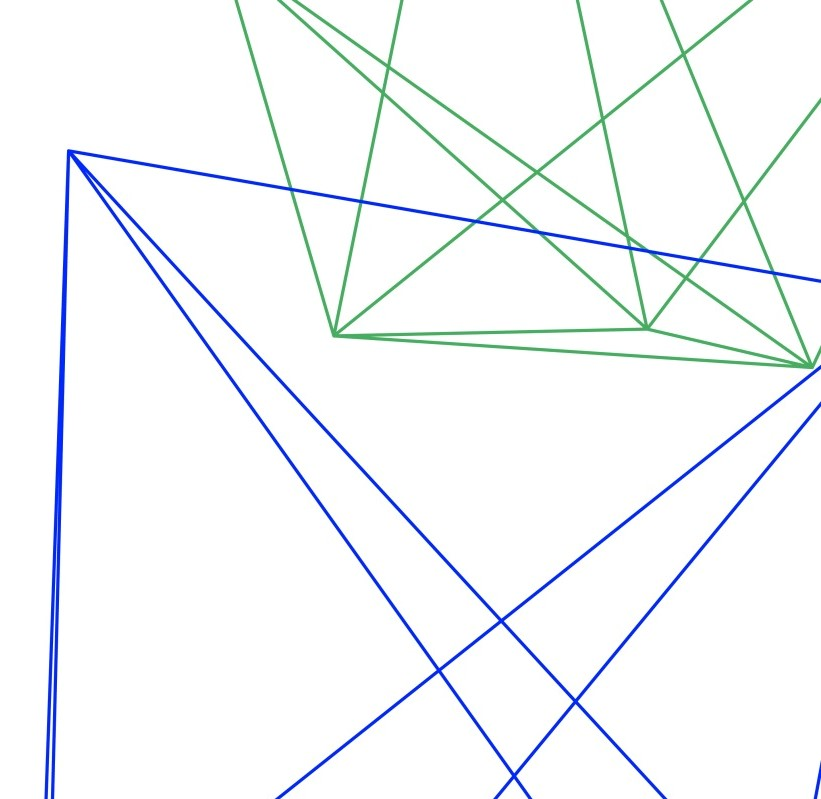
\includegraphics[width=0.5\paperwidth,height=\paperheight]{./logos/invert1.jpg}};

                \node[opacity=0.15, inner sep=0pt, anchor=south west] at (current page.south west){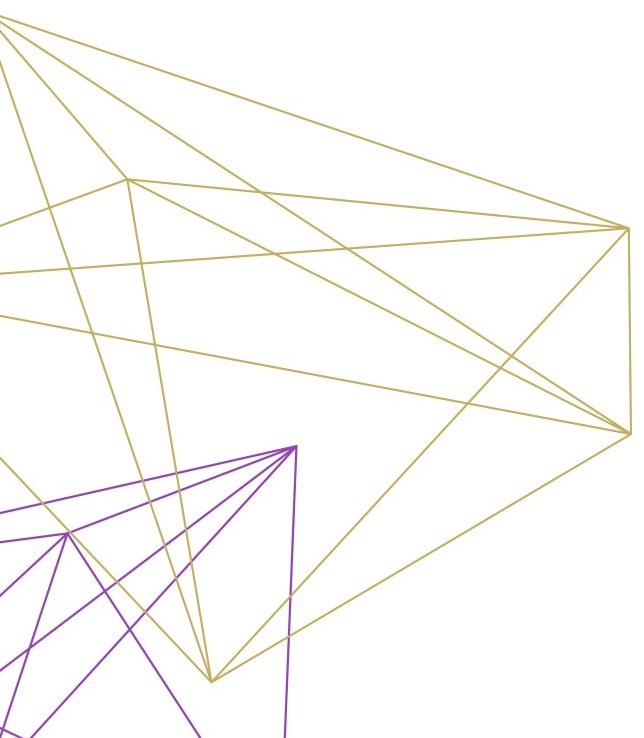
\includegraphics[width=0.5\paperwidth,height=0.5\paperheight]{./logos/invert2.jpg}};

                \node[opacity=0.15,inner sep=0pt, anchor=north west] at (current page.north west){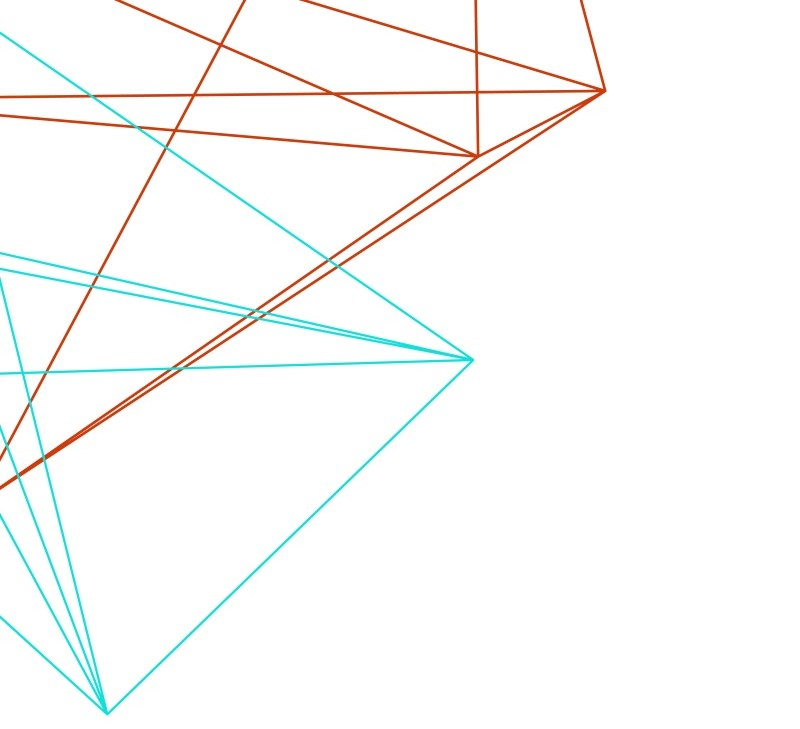
\includegraphics[width=0.5\paperwidth,height=0.5\paperheight]{./logos/invert3.jpg}};

                \node at (page cs:0,0.9) {
\includegraphics[height=1cm]{./logos/IMT.png}\hspace{1.5cm}
\includegraphics[height=1.5cm]{./logos/UJM.png}};

                \node at (page cs:0,0.8) {\Large\textsc{Cycle Initial en Technologies de l'Information de Saint-Étienne}};

                \node at (page cs:0,0.5) {\HUGE\textbf{TP1 Réseaux}};
                \draw (page cs:0.5,0.45) -- (page cs:-0.5,0.45); 

                \node at (page cs:0,0.4) {\Large\textsc{Lucas Lescure}}; 

                \node[opacity=0.5] at (page cs:-0.7,-0.8) {
\includegraphics[width=1.2\textwidth]{./logos/Logo-t.png}};

            \end{tikzpicture}          
        \end{titlepage}


    \newgeometry{width=18.625cm, bottom=2cm, top=2cm}

    \tikz[remember picture, overlay] \node[opacity=0.3,inner sep=0pt, anchor=north east] at (current page.north east){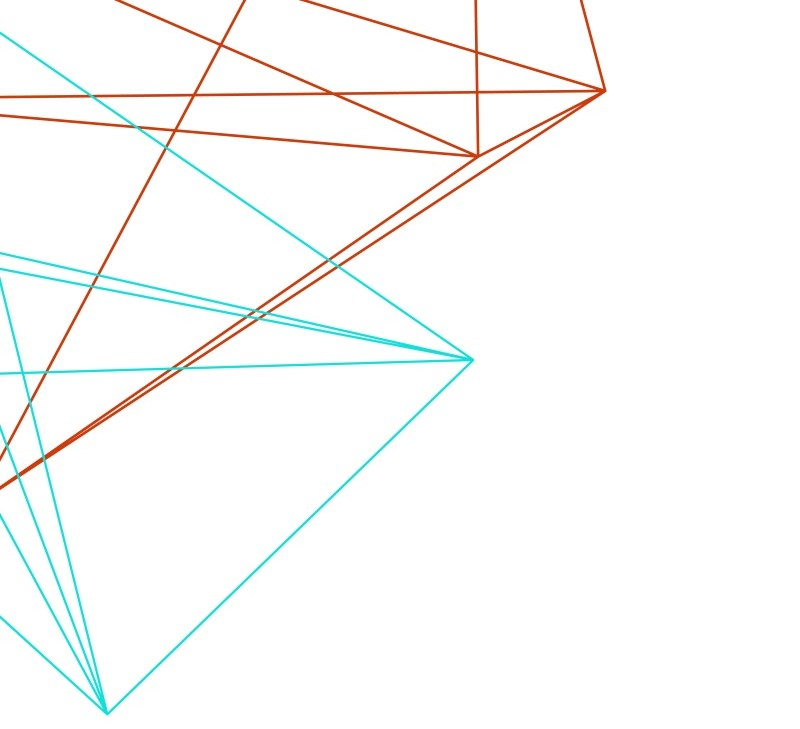
\includegraphics[angle=-90,origin=c,width=0.5\paperheight,height=0.5\paperwidth]{./logos/invert3.jpg}};
    \tikz[remember picture,overlay] \node[opacity=0.3,inner sep=0pt, anchor=south east] at (current page.south east){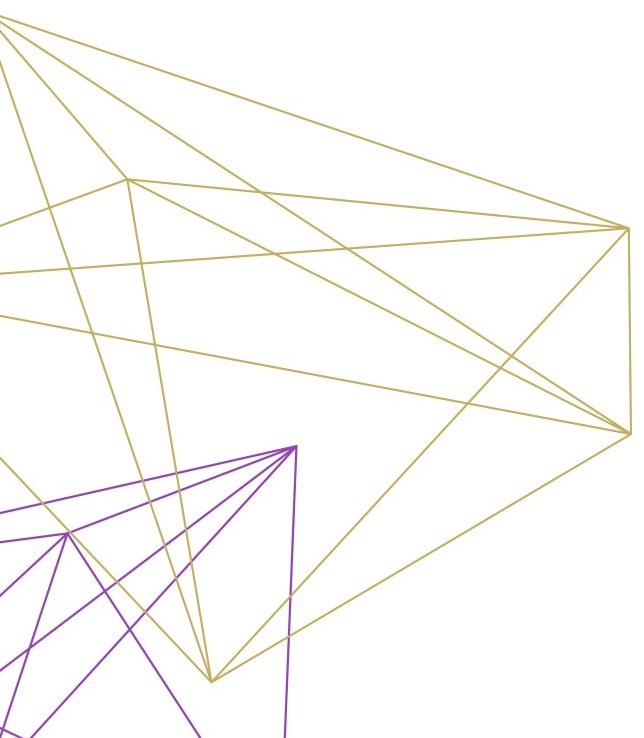
\includegraphics[angle=90,width=0.5\paperwidth,height=0.5\paperheight]{./logos/invert2.jpg}};

    \tableofcontents


    \newpage

    \section{Exercise 1}

        \begin{dent}{Q1 :} Quels types de câbles peut-on utiliser?\\
            Nous avons le choix entre 4 types de cables différents: 
            \begin{items}{-15pt}{-15pt}
                \item Paire de cables torsadées droit 
                \item Paire de cables torsadées croisé
                \item Câble coaxial
                \item Ligne telecom
            \end{items}
            On voit qu'avec la paire de cables torsadée droit, et ligne telecom il n'y a pas de trasnmission entre les deux machines, alors que pour la paire de cable torsadées croisé et le cable coaxial il y a une trasnmission entre les deux machines.
         \end{dent}

        \begin{dent}{Q2 :} Que se passe-t-il quand un système émet vers l'autre(broadcast-unicast)? Que se passe-t-il quand les 2 systemes émettent l'un vers l'autre\\
            \begin{enum}{-15pt}{-15pt}
                \item[a.] Lorsqu'une machine emet une trame, celle-ci est émise à la deuxième machine dans son réseau. De même avec une transmission \texttt{unicast}.
                \item[b.] Avec une paire torsadé croisé on voit que les deux trames s'envoi sur un fil différent il n'y a pas de collision de la trame. Avec une paire de cable coaxial on voit que ces deux trames sont transmises sur un même fil, il y a donc une collision. Les deux machines attendes un moment aléatoire avant que l'une d'elle ne renvoi la trame. S'il n'y a pas encore une collision, la première trame est transmise en premier, puis une fois finie, la deuxième trame est envoyée. 
            \end{enum}
         \end{dent}

        \begin{dent}{Q3 :} Après avoir vider les tables ARP de chaque machine, on effectue un ping de \texttt{st1} à \texttt{st2}\\
            Quelles sont les trames mises en oeuvre lorsque \texttt{st1} fait un ping vers \texttt{st2}?\\
            Quelle est la différence si on renouvelle ce ping (cache ARP)?
            \begin{enum}{-15pt}{-15pt}
                \item[a.] \texttt{st1} verifie sa table de routage pour savoir où envoyer la trame. Ensuite il envoi une requête ARP en broadcast vers tout les appareil. Quand \texttt{st2} reçois la trame il cherche l'IP source dans son cache, puisqu'elle n'y est pas, il rajoute l'IP avec l'addresse mac associé. Il examine ensuite la trame pour savoir si elle lui est déstinée puis après avoir traité la trame il la renvoi une réponse ARP à la machine \texttt{st1}. Celle-ci ne reconnais pas la source et l'ajoute donc dans son cache. Après traitement du signal elle envoi une tramme IP "\texttt{echo}" qui ping la machine \texttt{st2}, qui la renvoi ensuite après avoir traité et reconnue l'addresse source. Le paquet \texttt{EchoResponse} est lu par \texttt{st1} il sait donc que sont ping à bien été trasnmis. 
                \item[b.] Quand leur table ARP est déjà remplie, c'est à dire que les deux machine se connaissent, il n'y a pas de requête ARP, on passe directement à l'envoi de la trame \texttt{echo} par transmission IP.
            \end{enum}
         \end{dent}
        
    \section{Exercise 2 : Plusieurs systèmes raccordés par un HUB}
        
        \begin{dent}{Q1 :} Quel type de câble peut-on utiliser?\\
            On ne peut utiliser que la paire de cable torsadée droit. (dire pk)
         \end{dent}

        \begin{dent}{Q2 \& Q3 :} Quels systèmes reçoivent la trame(\texttt{broadcast}/\texttt{unicast}), et lesquelles la traitent?
            Lorsque l'on envoi une trame en \texttt{broadcast}, cette trame atteint toutes les machines liés au HUB, et elle est lu par tout le monde. En \texttt{unicast}, tout le monde reçois mais seulement la machine déstinataire lit le message transmis.     
         \end{dent}
        
        \begin{dent}{Q4 :}
            Lorsque l'on a deux machines qui envoi simultanément une trame, lorsque les deux trames atteignent le HUB, il y a collision sur toutes les autres transmission. On attend un temps aléatoire avant que l'une n'envoi sa trame, s'il n'y a pas encore de collision alors la deuxième envera sa trame une foit que la première se fasse traiter. 
         \end{dent} 
        
    \section{Exercise 3 : Plusieurs systèmes raccordés par un SWITCH}
        
        \begin{dent}{Q1 :} Quel type de cable faut-il utiliser?\\
            Comme dans l'exercise précédent on doit utiliser le cable torsadée droit
         \end{dent}

        \begin{dent}{Q2 :} Différence entre "on the fly" et "store and forward"\\
            \begin{enum}{-15pt}{-15pt}
                \item[a.] Lorsque l'on met le switch en mode "on the fly" on voit que les trames sont à la fois routés vers le réseaux et sauvegardées en mémoire par la switch pour être sur qu'il n'y ai pas de collision sur les transmissions.  
                \item[b.] En mode "store and forward" il atteind d'avoir reçu la trame entièrement avant de les réenvoyer sur les machines du réseau, on évite aussi les collision entre les trames. 
            \end{enum}
         \end{dent}

        \begin{dent}{Q3 :} On affiche la table MAC/Port du switch :
            \begin{figure}[ht]
                \centering
                \begin{tabular}{c|c|c}
                    Addresse & Port & TTL\\
                    \hline
                    MAC01 & 1 & Elevé \\
                    \hline
                    MAC02 & 2 & Elevé \\
                    \hline
                    MAC03 & 3 & Elevé \\
                    \hline:
                    MAC04 & 4 & Elevé \\
                \end{tabular}
                \caption{\ul{Table MAC/Port SWITCH}}
            \end{figure}
         \end{dent}
        
         \begin{dent}{Q4 \& Q5:} Que fait le switch?\\
            Le switch transmet directement d'une machine à l'autre agissant comme un pont, seulement la machine déstinée recoit la trame:op
             
          \end{dent}
         

        \begin{dent}{Q7 :} On affiche la table MAC/Port suite aux 3 transmissions:
            \begin{figure}[ht]
                \centering
                \begin{tabular}{c|c|c}
                    Addresse & Port & TTL\\
                    \hline
                    MAC01 & 1 & Elevé \\
                    \hline
                    MAC03 & 3 & Moyen \\
                \end{tabular}
                \caption{\ul{Table MAC/Port SWITCH}}
            \end{figure}
         \end{dent}
        



\end{document}